% !TeX spellcheck = en_GB
\documentclass[12pt,fleqn]{article}

\usepackage[english]{babel}
\usepackage{SpeedyGonzales}
\usepackage{MediocreMike}
%\usepackage{Blastoise}

\title{}
\author{Asger Schultz}
\date{\today}

\fancypagestyle{plain}
{
	\fancyhf{}
	\rfoot{Side \thepage{} af \pageref{LastPage}}
	\renewcommand{\headrulewidth}{0pt}
}
\pagestyle{fancy}
\fancyhf{}
\lhead{Asger Schultz}
\chead{}
\rhead{}
\rfoot{Side \thepage{} af \pageref{LastPage}}

\graphicspath{{Billeder/}}
\linespread{1.15}


%\numberwithin{equation}{section}
%\numberwithin{footnote}{section}
%\numberwithin{figure}{section}
%\numberwithin{table}{section}

\begin{document}

\maketitle
%\thispagestyle{fancy}
%\tableofcontents
-- Compare measurement methods of bioavailable phosphorous and examine the influence of bioavailable phosphorous on harvest yield. 
-- By the explanatory strengths of the two measurements, the DGT measurement is found to be most useful in predicting the yield.
-- Bioavailable phosphorous is using both measurements found to have significant effect on the yield \(p<10^{-9}\).
\tableofcontents
\newpage 
\section{Introduction}
A wide range of very different effects are in play in determining the output yield of a farm.
As environmental and economic incentives rise, there is increasing motivation for precision agriculture which optimizes the performance of farming using ecological, chemical and biological variables.
One of these important variables is the nutrient of the soil and \textit{phosphorous} is essential in this regard.


This report considers different techniques for measuring the amount of phosphorous available to the plants and compares two measurement methods, the traditional "Olsen-P" and the newer "DGT" method, using the output yield of barley fields as the target.  
Correlations, model fitting of Michaelis-Menten models and ANCOVA models are used to examine the connections between the measurements and the yield output.
\section{Data}
The data consists of 100 observations each consisting continuous  Olsen-P measurements [mg/100g], DGT-measurements [\(\mu\)g/L] and harvest yield of barley [hkg/ha] and categorical location id's for the field on which the observations were made. Nine fields have been surveyed and given id's from "001" to "011". The last field has missing values for two of it's three yield measurements.  

The fields are from Denmark and Norway and the multiple measurements of yield from each field correspond to division of the fields into plots from which soil samples were taken and later barley output was recorded such that these measurements cannot be considered independent which is visualized in below boxplot. Further visualization of the data is given in the results section where scatter plots are supplied.
\begin{figure}[H]
	\centering
	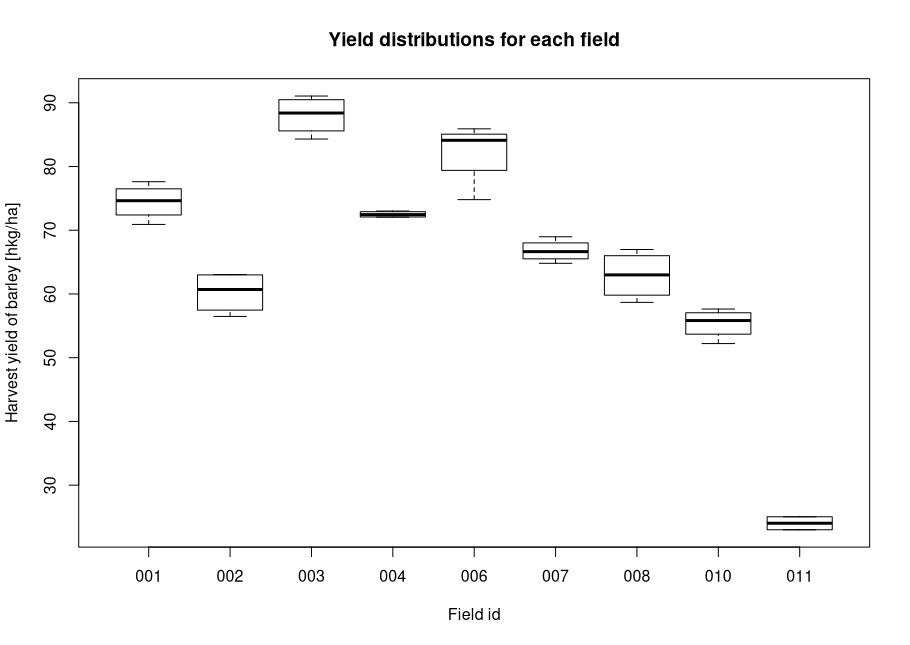
\includegraphics[width=.7\linewidth]{p2_fieldbox}
	\caption{Boxplot of the barley output measurements for the plots in each field. Note the much larger between-field variance than within-field variance which shows that the multiple observations on the same field cannot be considered independent.}
\end{figure}
\section{Methods and analysis}
\subsection{Recommended measure}
Without access to a verifiable measurement of bioavailable phosphorous, the measurement methods are evaluated based on their ability to explain, and thus, predict the yield of the field. 

As an initial examination, the correlation between yield output and each phosphorous measurement is found and visualized to account for linear relationships. The correlation between the two measurements is also included together with visualizations of the significance of the correlations.

To test which measurement predicts the barley yield best beyond linear tendencies, Michaelis-Menten models are used. The nonlinear model is connected to the reaction velocity of enzymes such as nutrients \cite{michment} and assumes that:
\[
y = \frac{\alpha x}{\beta + x}, x >0
\]
This nonlinear model is fitted using the yield as target variable and both DGT measurements and Olsen P-measurements as explanatory variables by the R function \texttt{nls} which iteratively fits the parameters using a squared loss criterion.  To estimate the generalization error of each model, leave-one-out cross-validation over the fields is performed by fitting the models to eight out of the nine and evaluating them on the last for all fields. The starting guesses for each model is kept constant.

From this, estimates of the two model's generalization errors as the mean squared error loss are found and these are compared with a t-test on test errors of the nine folds to evaluate the evidence for the hypothesis that modelling using one measurement technique is better than using the other.
\subsection{Yield influence of bioavailable phosphorous}
To test whether there is a significant effect of bioavailable phosphorous on the barley yield, ANCOVA models of the following form is evaluated:
\[
y = \alpha_{field, i} + \beta x
\]
where \(y\) is the barley yield and two models are evalued with \(x\) being the DGT and the Olsen-P measurements respectively. Interaction effects are not included due to the missing data in one of the fields such that only one slope is evaluated for each model. The significance of this slope is then evaluated using the ANCOVA F-test for each model.
\section{Results}
\begin{figure}[H]
	\centering
	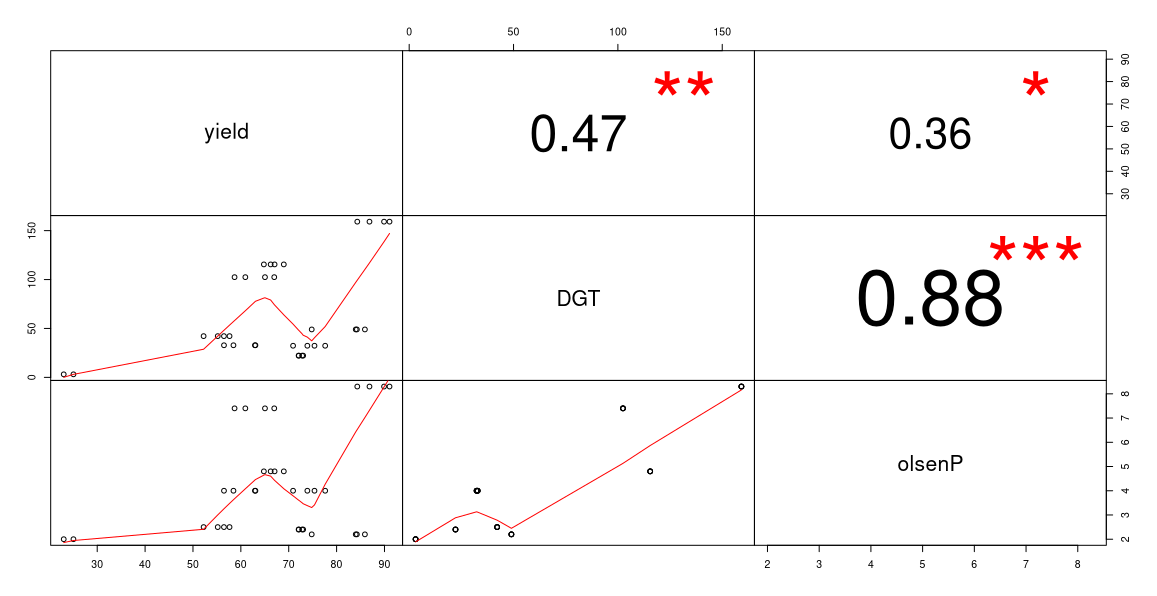
\includegraphics[width=.9\linewidth]{p2_corrplot}
	\caption{Visualization of a Correlation Matrix. On top the (absolute) value of the correlation plus the result of the cor.test as stars. On bottom, the bivariate scatterplots, with a fitted line}
\end{figure}
\begin{figure}[H]
	\centering
	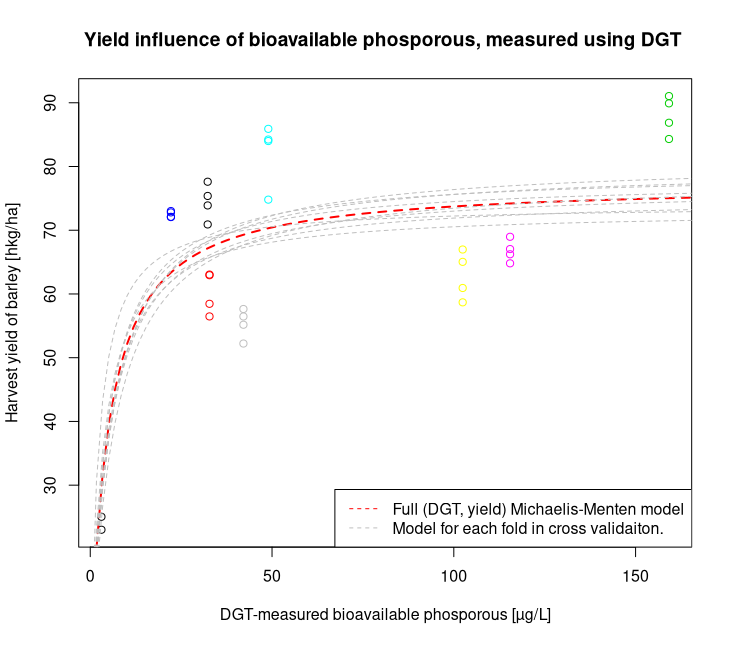
\includegraphics[width=.8\linewidth]{dgt_mmm}
\end{figure}
\begin{figure}[H]
	\centering
	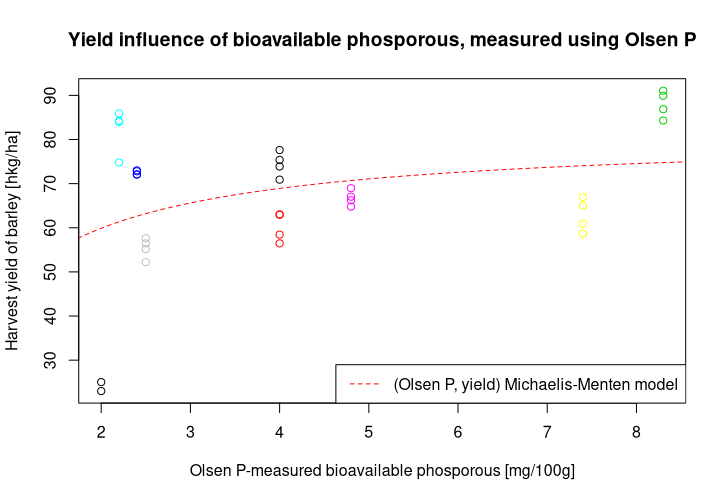
\includegraphics[width=.8\linewidth]{oP_mm}
\end{figure}

\begin{align*}
	& \sqrt{MSE_{dgt}}	 = 10.84
	&& \sqrt{MSE_{olsenP}} = 14.65
\end{align*}
%\begin{figure}[H]
%	\centering
%	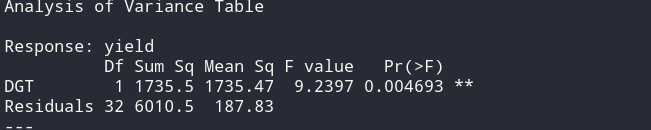
\includegraphics[width=.7\linewidth]{simpleDGT}
%\end{figure}



%\begin{figure}[H]
%	\centering
%	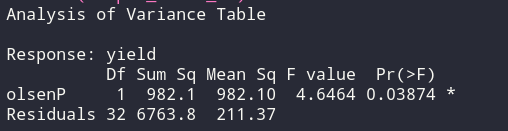
\includegraphics[width=.7\linewidth]{simpleOP}
%\end{figure}
\begin{figure}[H]
	\centering
	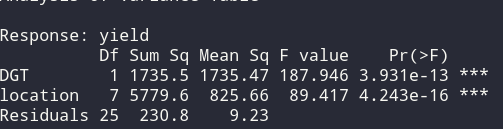
\includegraphics[width=.7\linewidth]{anovaDGT}
\end{figure}
\begin{figure}[H]
	\centering
	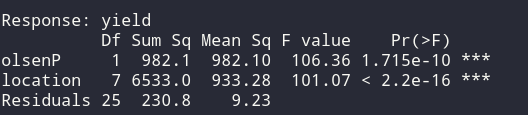
\includegraphics[width=.7\linewidth]{anovaOP}
\end{figure}

\section{Discussion}
\begin{thebibliography}{9}
	\bibitem{michment}Dragan, J., Kristian, S., Scitovski, R.: "Total least squares fitting Michaelis–Menten enzyme kinetic model function", 04-07, Journal of Computational and Applied Mathematics, 201:1. 

\end{thebibliography}
\end{document}

















